
%%%%%%%%%%%%%%%%%%%%%%%%%%%%%%%%%%%%%%%%%%%%%%%%%%%%%%%%%%%%%%%%%%%%%%%%%%%%%%%
\begin{frame}[fragile]{Benchopt \rightcite{Moreau et al. 2022}}

Reproducing this comparison and adding solvers and tasks is easy as:\\[.5em]


\begin{center}
\begin{tabular}{c}
\begin{lstlisting}[language=bash,linewidth=.85\textwidth]
git clone https://github.com/benchopt/benchmark_bilevel
benchopt run ./benchmark_bilevel
\end{lstlisting}
\end{tabular}
\end{center}

\vskip.5em\centering
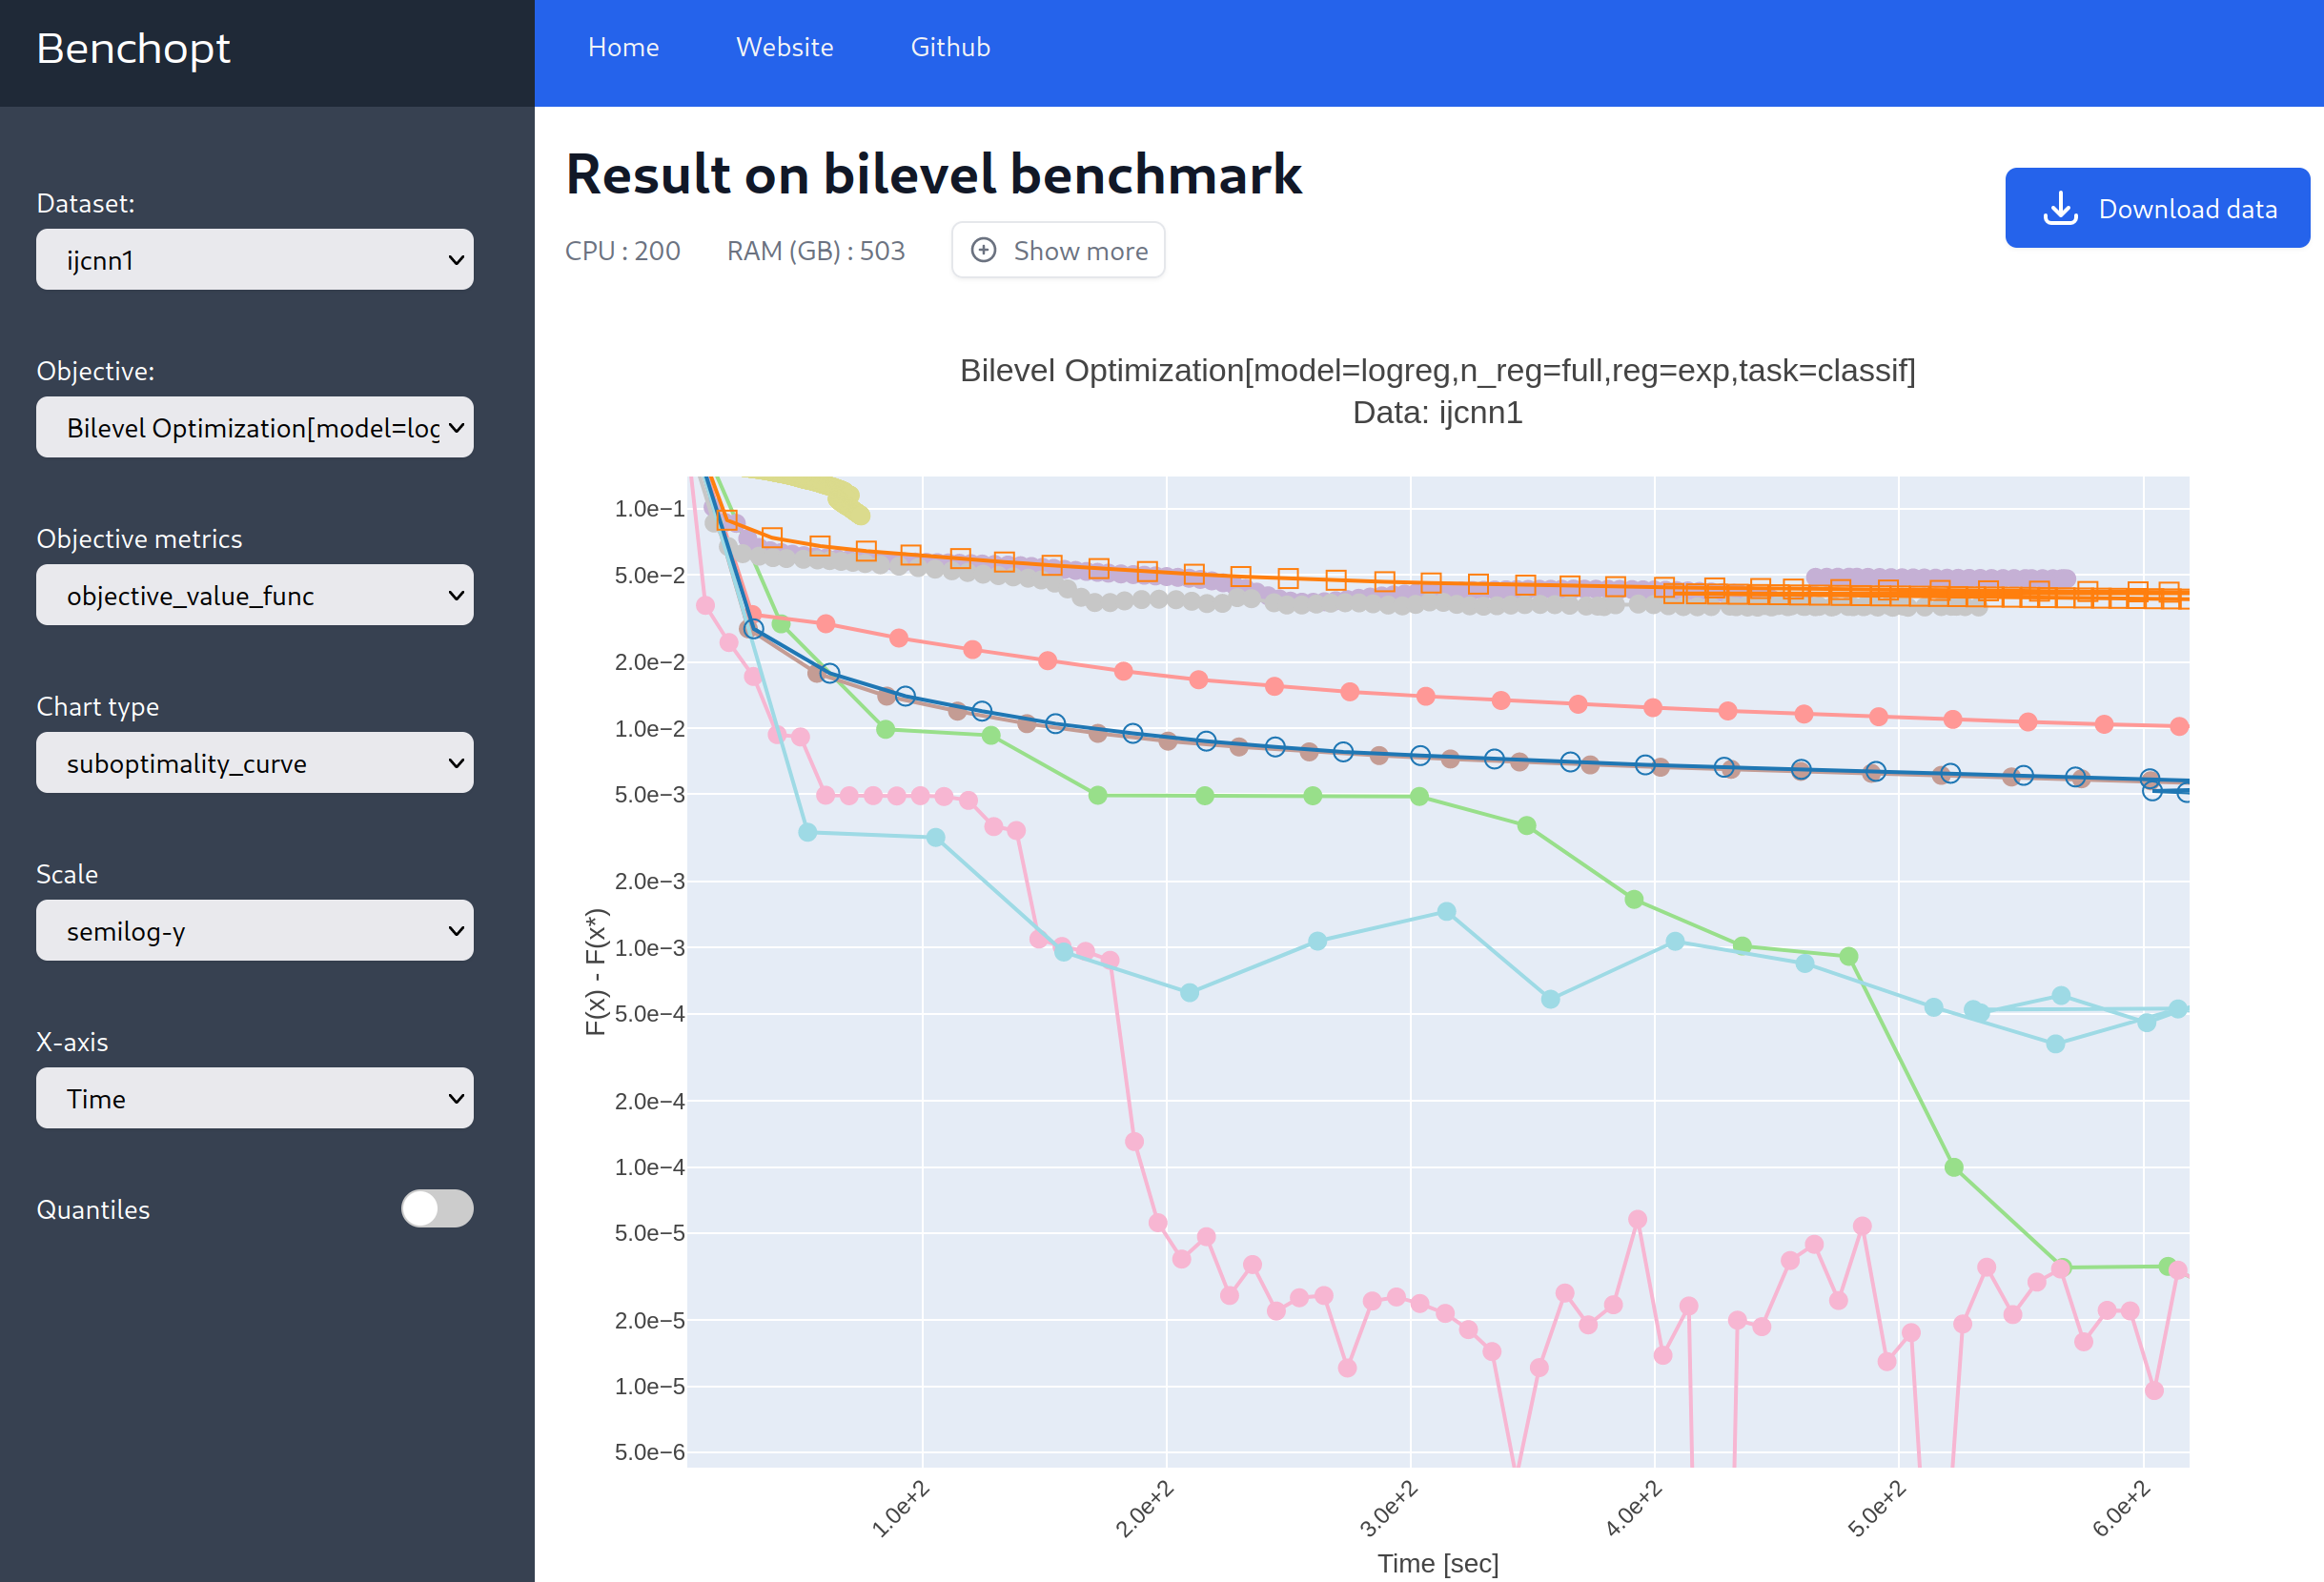
\includegraphics[width=.7\textwidth]{benchopt_bilevel}\\

% \hskip3ex
% 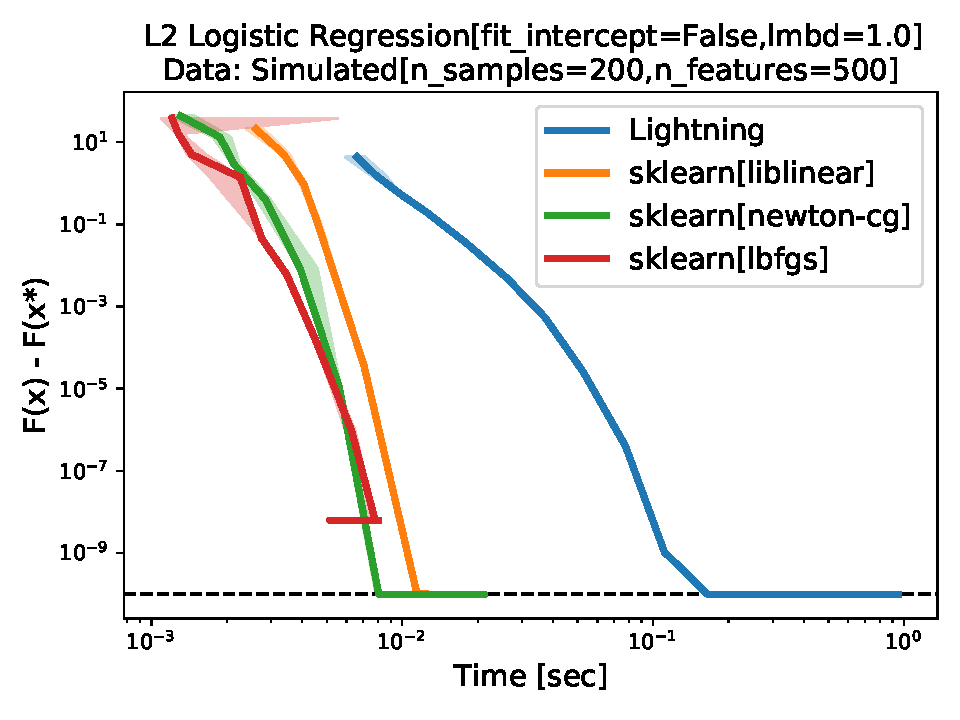
\includegraphics[width=.45\textwidth]{logreg_l2_1}

\end{frame}
%%%%%%%%%%%%%%%%%%%%%%%%%%%%%%%%%%%%%%%%%%%%%%%%%%%%%%%%%%%%%%%%%%%%%%%%%%%%%%%


%%%%%%%%%%%%%%%%%%%%%%%%%%%%%%%%%%%%%%%%%%%%%%%%%%%%%%%%%%%%%%%%%%%%%%%%%%%%%%%
\begin{frame}{Benchopt principle}

A benchmark is a directory with:\\
\begin{itemize}
    \item An \lstinline+objective.py+ file with an \lstinline+Objective+ that define the metrics.
    \item A directory \lstinline+datasets+ with \lstinline+Dataset+ that define inner and outer tasks.
    \item A directory \lstinline+solvers+ with one file per \lstinline+Solver+
\end{itemize}
\vskip1em

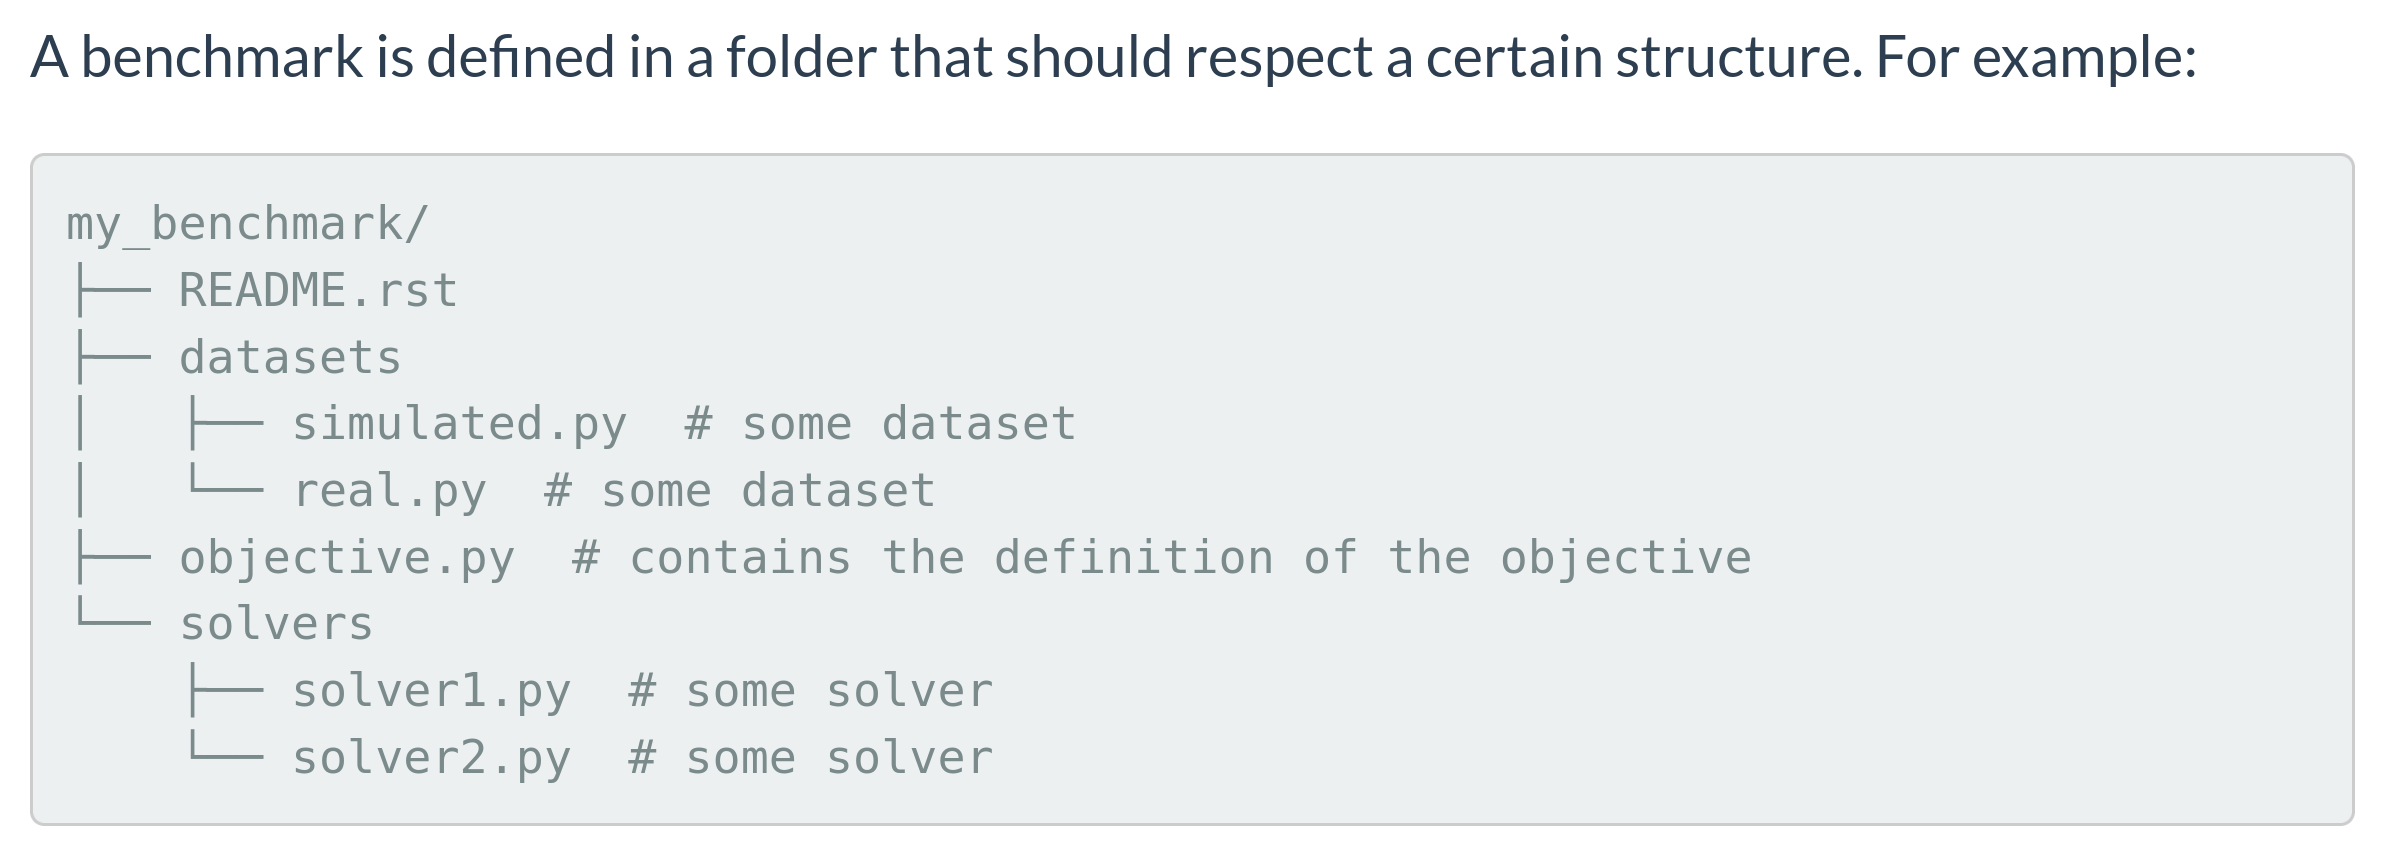
\includegraphics[width=.9\textwidth,trim={0 0 0 2.8em},clip]{benchopt_structure}

\vskip1em
The \lstinline+benchopt+ client runs a cross product and generates a parquet file + HTML visualisation to explore the results.
\end{frame}
%%%%%%%%%%%%%%%%%%%%%%%%%%%%%%%%%%%%%%%%%%%%%%%%%%%%%%%%%%%%%%%%%%%%%%%%%%%%%%%

%%%%%%%%%%%%%%%%%%%%%%%%%%%%%%%%%%%%%%%%%%%%%%%%%%%%%%%%%%%%%%%%%%%%%%%%%%%%%%%
\frame{
    \frametitle{Benchopt: principle}

    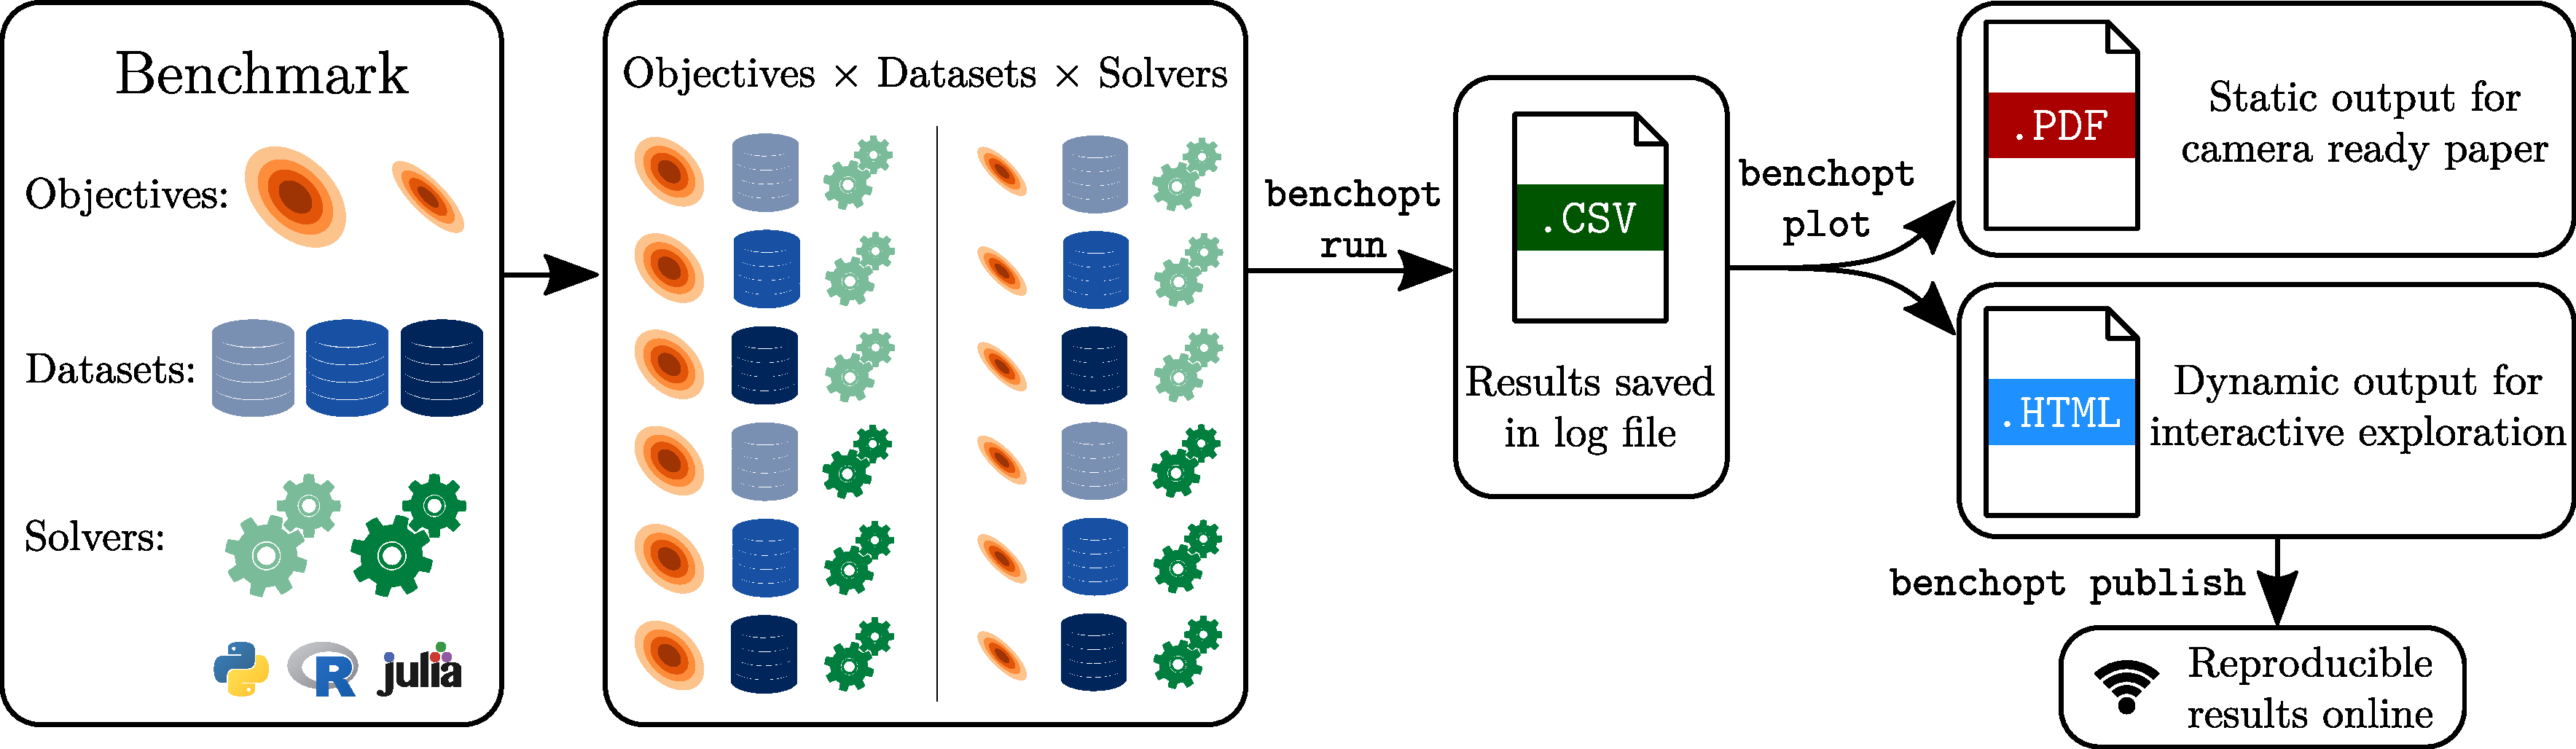
\includegraphics[width=\textwidth]{benchopt_schema_objectives_with_logos}

    \strongpoint{Each object can be parametrized so multiple scenario can be tested.}

    \vskip1.5em
    \textbf{Making tedious tasks easy:}\\[1em]
    \centering

    \myitem{} Sharing code
    \hskip3ex \myitem{} Adding methods
    \hskip3ex \myitem{} Exploring results\\[.5em]
    \myitem{} Varying hyperparameters
    \hskip3ex \myitem{} Running in Parallel
    \hskip3ex \myitem{} Caching\\[.5em]
    \hskip-4em\myitem{} \dots
}


%%%%%%%%%%%%%%%%%%%%%%%%%%%%%%%%%%%%%%%%%%%%%%%%%%%%%%%%%%%%%%%%%%%%%%%%%%%%%%%
